\chapter{User Documentation} % User guide
\label{ch:user}


In this chapter, the Clang Static Analyzer will be explained from an end-user perspective. Clang SA is a Clang compiler library that can be found in the LLVM project repository \cite{llvm-project}. 

This work implements two new checkers, \emph{alpha.security.cert.pos.34c} for POS34-C and \emph{alpha.security.cert.env.InvalidPtr} to cover both ENV31-C and ENV34-C. At the time of writing, the first checker is already included in LLVM, while the second is still undergoing official review. 


\section{Install Guide}


\subsection{System Requirements}
Table \ref{tab:sys-req} shows the system requirements and supported compilers for building LLVM. The checkers were developed with Ubuntu 20.04 and tested on Ubuntu 18.04, macOS, and WSL Ubuntu 20.04.


\begin{table}[H]
	\centering
	\begin{tabular}{ | m{0.25\textwidth} | m{0.25\textwidth} | m{0.25\textwidth} |}
		\hline
		\textbf{Operating System} & \textbf{Processor Architecture} & \textbf{Compiler} \\
		\hline \hline
		Linux & x861 & gcc, clang\\
		\hline
		Linux & amd64 & gcc, clang\\
		\hline
		Linux & arm & gcc, clang\\
		\hline
		Linux & Mips & gcc, clang\\
		\hline
		Linux & PowerPC & gcc, clang\\
		\hline
		Solaris & V9 & gcc\\
		\hline
		FreeBSD & x861 & gcc, clang\\
		\hline
		FreeBSD & amd64 & gcc, clang\\
		\hline
		NetBSD & x861 & gcc, clang\\
		\hline
		NetBSD & amd64 & gcc, clang\\
		\hline
		macOS2 & PowerPC & gcc\\
		\hline
		macOS & x86 & gcc, clang\\
		\hline
		Cygwin & x86 & gcc\\
		\hline
		Windows & x86 & Visual Studio\\
		\hline
		Windows64 & x86-64 & Visual Studio\\
		\hline
	\end{tabular}
	\caption{Clang Static Analyzer system requirements}
	\label{tab:sys-req}
\end{table}

\subsection{Building from source}


The commands below will compile LLVM from source. Note that prerequisites are \emph{git}, \emph{CMake} (version 3.4.3 or higher), \emph{gcc} (version 5.1.0 or higher), and \emph{Ninja} build system \cite{ninja}.

\begin{lstlisting}[caption={},label={lst:llvm-build1}]
# on Windows --config core.autocrlf=false flag need to be added to the git clone command.
git clone https://github.com/llvm/llvm-project.git
cd llvm-project

# POS34 checker is already part of LLVM, however for ENV checker user needs to apply git patch
# on top of c79bc5942d0efd4740c7a6d36ad951c59ef3bc0e
# Author: Stefan Pintilie <stefanp@ca.ibm.com>, Date: Tue May 11 05:32:32 2021 -0500
# It could work with the current HEAD of llvm-project, but recent changes might have caused merge conflict.

git checkout c79bc5942d0efd4740c7a6d36ad951c59ef3bc0e
git apply ../invalidPtrChecker.diff

mkdir build
cd build

# Configure build using cmake
cmake \
      -G "Ninja" \
      -DLLVM_ENABLE_PROJECTS="llvm;clang;clang-tools-extra" \
      -DCMAKE_BUILD_TYPE=Release \
      -DBUILD_SHARED_LIBS=ON \
      -DLLVM_TARGETS_TO_BUILD=X86 \
      -DCMAKE_EXPORT_COMPILE_COMMANDS=ON \
      ../llvm/

# -j 4 is number of parallel jobs, user can set it to more.
# It will take a while...
ninja -j 4

# For ease of use the user can add built binaries to the PATH
# export PATH="path/to/llvm-project/build/bin:$PATH"
\end{lstlisting}


\section{Running Analysis} \label{run-analysis}
To demonstrate how to use Clang Static Analyzer, we create main.c file with the following code:

\lstset{caption={}, label=src:trial_run}
\begin{lstlisting}[language={C++}]
#include <stdlib.h>
#include <stdio.h>

int call_putenv(const char *var) {
  char env[1024];
  int retval = snprintf(env , sizeof(env), "TEST=%s", var);
  if (retval < 0) {
    // handle error
  }
  return putenv(env); // putenv function should not be called with auto variables
}

int main(){
  call_putenv("hello clang!");
}
\end{lstlisting}

The simplest way to run Clang SA is to use the clang compiler with the \lstinline{--analyze} option. In order to activate our checkers, we must also include \lstinline{-analyzer-checker=<checker name>} flag. 



\begin{lstlisting}[caption={},label={lst:running-pos34},language={bash}]
clang main.c --analyze \
 -Xclang -analyzer-checker=alpha.security.cert.pos.34c
\end{lstlisting}

If the installation was successful, running the above command gives the following output:

\begin{figure}[H]
	\centering
	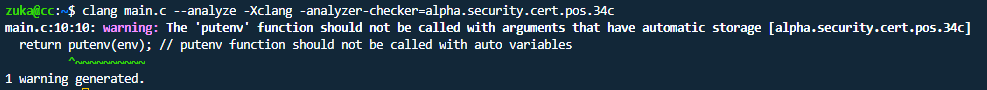
\includegraphics[width=\textwidth]{images/new_pos34.PNG}
	\caption{POS34-C checker output}
	\label{fig:pos34termin}
\end{figure}


Similarly to the POS34-C, the following command can be used to check for ENV31 and ENV34 violations: 
\begin{lstlisting}[caption={},label={lst:running-env}]
clang main.c --analyze \
 -Xclang -analyzer-checker=alpha.security.cert.env.InvalidPtr
\end{lstlisting}

\section{Output options}
More analyzer-specific flags can be added to the invocation commands seen in \ref{run-analysis}.
Users, for example, can choose the best output format for their needs: 
\begin{lstlisting}[caption={},label={lst:output-flag}]
clang main.c --analyze \
 -Xclang -analyzer-checker=alpha.security.cert.env.InvalidPtr \
 -Xclang -analyzer-output=<output type>
\end{lstlisting}

Running the command without the \lstinline{analyzer-output} flag results in default value "none", i.e. it gives warning in standard output as shown in figure \ref{fig:pos34termin}.

\subsection{Text output} \label{text-output}

\lstinline{-analyzer-output=text} still displays the analysis result in the terminal, but it also shows the path diagnostic messages.
Following the actual warning, we can see the steps taken by the symbolic execution that resulted in the bug. 

\begin{figure}[H]
	\centering
	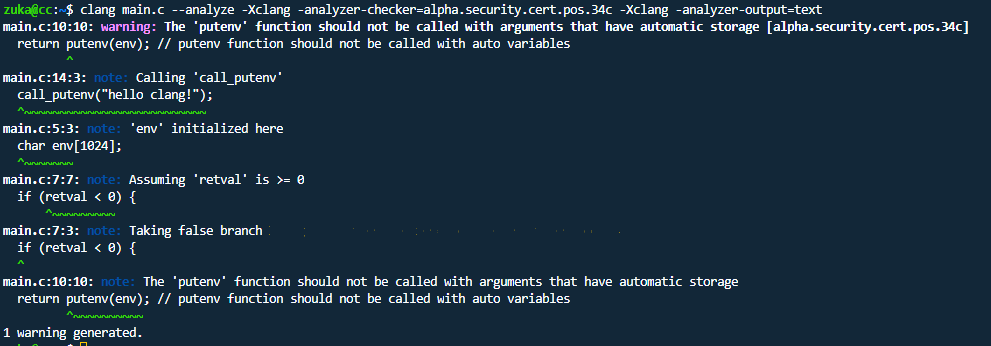
\includegraphics[width=\textwidth]{images/text.PNG}
	\caption{POS34-C with diagnostics}
	\label{fig:pos34termin2}
\end{figure}

\subsection{HTML output} \label{html-output}
The analysis results can also be viewed in HTML format, with a simple graphical interface. 

\begin{lstlisting}[caption={},label={lst:html-output}]
clang main.c --analyze \
 -Xclang -analyzer-checker=alpha.security.cert.env.InvalidPtr
 -Xclang -analyzer-output=html
 -o output/
\end{lstlisting}

If we run the above command will create a new "output" directory (if one does not already exist) where the analysis results will be stored. In our case, it will generate a single (depending on the number of warnings in our source code) HTML file, which will look like this when viewed in a browser: 

\begin{figure}[H]
	\centering
	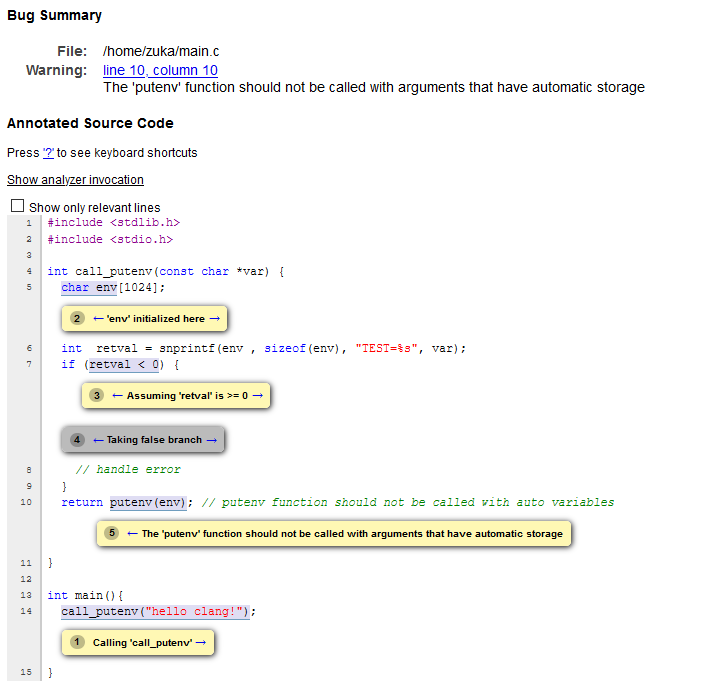
\includegraphics[width=\textwidth]{images/html_out.PNG}
	\caption{HTML output example}
	\label{fig:html-output}
\end{figure}

\subsection{scan-build}
scan-build \cite{scan-build} is a command-line utility that acts as a wrapper around analysis invocation.

The command's general format is as follows: \\
\lstinline{scan-build [scan-build options] <command> [command options]} \\ 
It generates HTML reports and displays warnings in the terminal.

When \lstinline{-o} is not used to specify the output directory, it creates a temp folder with the current timestamp as the name by default. 

Running "scan-view" suggested at the last line of output will start webserver where analysis can be examined.


To browse the list of found bugs, a single index.html file is generated, and by opening a specific report, we see a page similar to figure \ref{fig:html-output}. 


\begin{figure}[H]
	\centering
	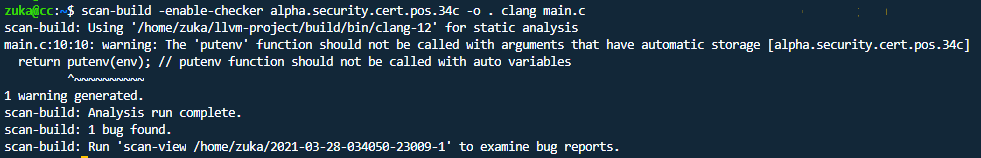
\includegraphics[width=\textwidth]{images/scan-build.PNG}
	\caption{scan-build output}
	\label{fig:scan-build}
\end{figure}


The main benefit of scan-build is that the second part of its invocation can contain any command, allowing users to run static analysis as part of performing a regular build, for example: \\ 
\lstinline{scan-build -enable-checker alpha.security.cert.env.InvalidPtr -o . make -j4} \\
Moreover, \lstinline{--use-analyzer=<path to clang>} flag can also be added, if the user wishes to use the specific clang build version.

\subsection{CodeChecker} \label{codechecker}
Ericsson developed the CodeChecker \cite{cc} tool in collaboration with Eötvös Loránd University to replace the scan-view utility.
In this section, we will show you how to use CodeChecker to analyze an open-source "git" project.

It should be noted that CodeChecker is only available for Linux and Mac OS. 


\subsubsection{Setting up CodeChecker}

To build the CodeChecker from source files, use the following commands: 
\begin{lstlisting}[caption={},label={}, language={bash}]
# prerequisites are npm, virtualenv

git clone https://github.com/Ericsson/CodeChecker.git --depth 1 ~/codechecker
cd ~/codechecker

# create virtual environment and activate it
make venv # or venv_osx for mac
source $PWD/venv/bin/activate

# build codechecker
make package

# optionally user can add it to path for ease of use:
# export PATH="$PWD/build/CodeChecker/bin:$PATH"

cd ..
\end{lstlisting}

\subsubsection{Configuring clang version}
CodeChecker detects and uses the latest available version of Clang that is in the user's path. Since we wish to use the custom-built clang for analysis, we must specify it inside configuration file \lstinline{~/codechecker/build/CodeChecker/config/package_layout.json} Value of "clangsa" should be set to \lstinline{/path/to/llvm-project/build/bin/clang}.


\subsubsection{Running analysis on git}

\lstset{caption={}, label=src:git1}
\begin{lstlisting}[language={bash}]
# install prerequisites for building git
sudo apt-get install gettext
git clone https://github.com/git/git.git
cd git
make configure
./configure --prefix=/usr
CodeChecker log -b "make all -j42" -o compile_commands.json
\end{lstlisting}

The commands above will generate a JSON file containing a compilation database for the git build process. This file is passed to the \lstinline{CodeChecker analyze}, which performs the analysis on each compile command.

\lstset{caption={}, label=src:git2}
\begin{lstlisting}[language={bash}]
CodeChecker analyze \
  /path/to/compile_commands.json \
  --analyzers clangsa \
  --enable alpha.security.cert.env.InvalidPtr \ 
  -o /path/to/output/dir/ \
  -j 42
\end{lstlisting}

This will generate analysis results in .plist files, which can then be converted to HTML with the \lstinline{CodeChecker parse} command. 

\begin{figure}[H]
	\centering
	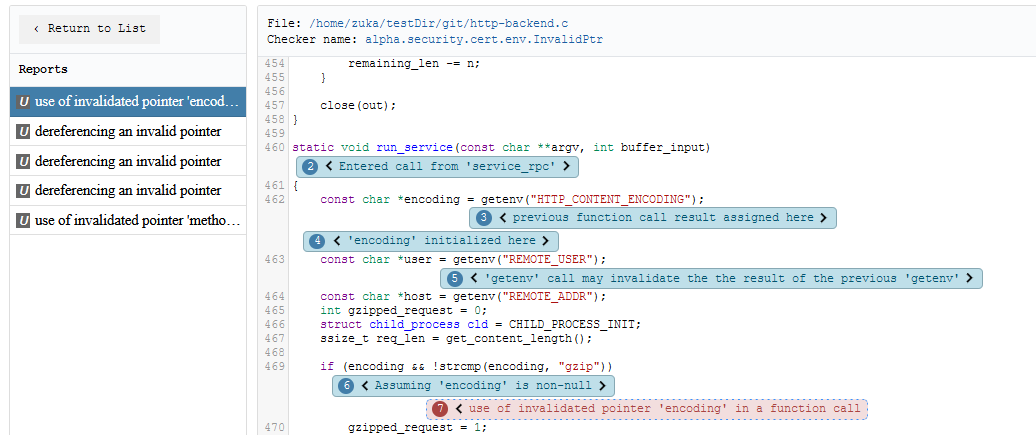
\includegraphics[width=\textwidth]{images/cc_html.PNG}
	\caption{CodeChecker html output}
	\label{fig:cc-html}
\end{figure}

CodeChecker allows users to save analysis results on its server, providing them with a sophisticated graphical interface. 

\lstset{caption={}, label=src:git3}
\begin{lstlisting}[language={bash}]
# start the server on localhost:8555/
CodeChecker server --workspace ./ws --port 8555

# store the analysis results in CC database
CodeChecker store \
  /path/to/plist/files/ \
  --name "project name" \
  --url http://localhost:8555/Default
\end{lstlisting}



\begin{figure}[H]
	\centering
	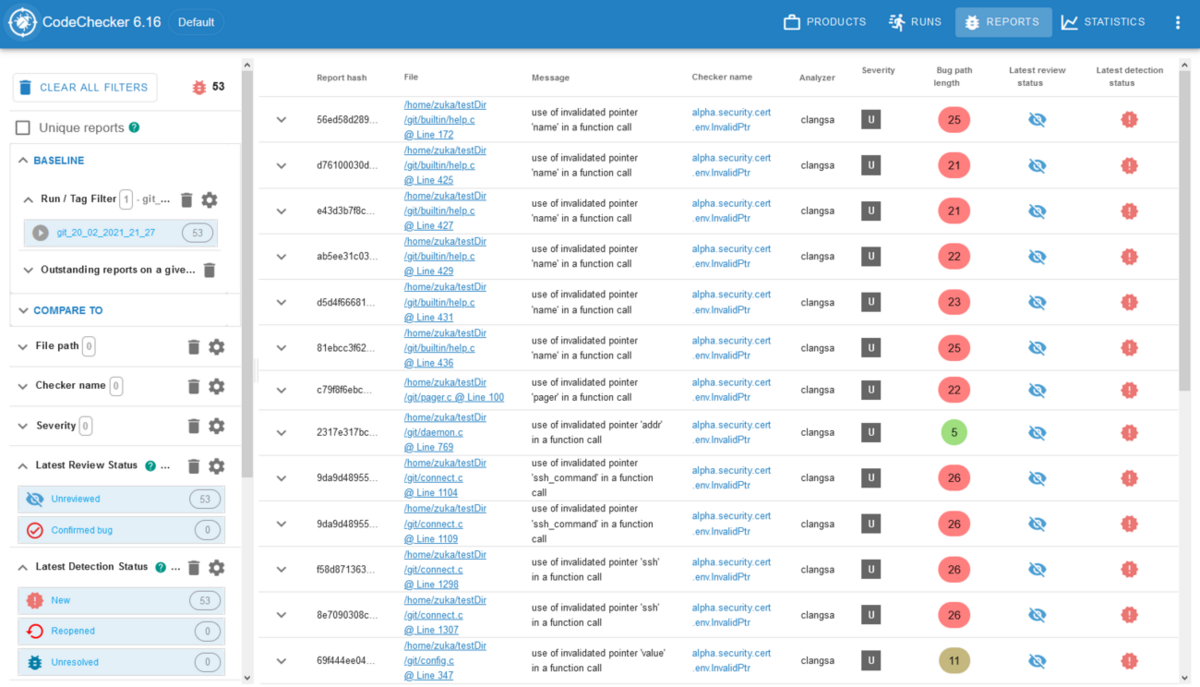
\includegraphics[width=\textwidth]{images/codechecker_reports_new_new.png}
	\caption{CodeChecker graphical user interface, list of reports}
	\label{fig:cc-reports}
\end{figure}

\begin{figure}[H]
	\centering
	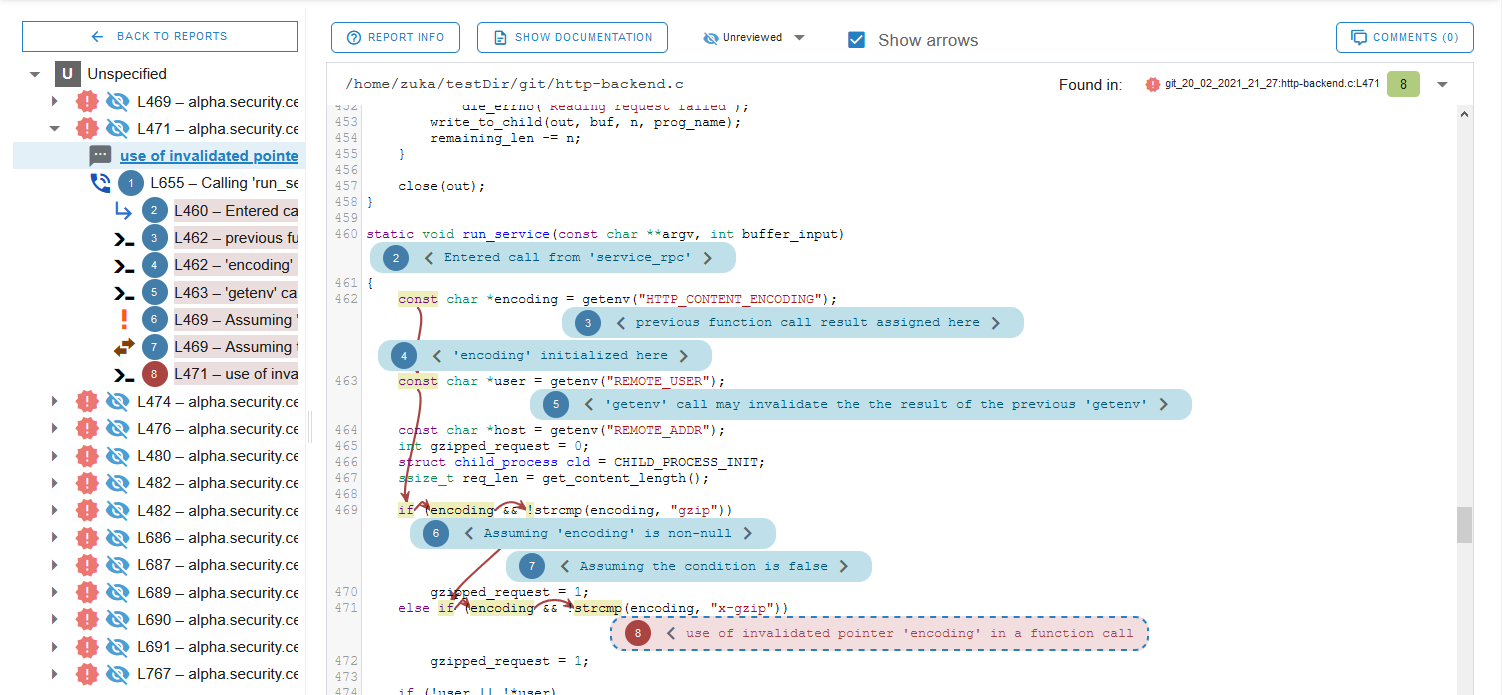
\includegraphics[width=\textwidth]{images/cc_path.PNG}
	\caption{CodeChecker graphical user interface, path diagnostics}
	\label{fig:cc-arrows}
\end{figure}
